% !TEX TS-program = XeLaTeX
% use the following command: 
% all document files must be coded in UTF-8
\documentclass{textolivre}
% for anonymous submission
%\documentclass[anonymous]{textolivre}
% to create HTML use 
%\documentclass{textolivre-html}
% HTML compile using make4ht
% $ make4ht -c textolivre-html.cfg -u -x article "fn-in,svg,pic-align"   
%
% See more information on the repository: https://github.com/leolca/textolivre

% Metadata
\begin{filecontents*}[overwrite]{article.xmpdata}
    \Title{Marketing digital y posicionamiento web en comunicación científica: a propósito de un caso en el área de Comunicación}
    \Author{Sara Mandiá Rubal \sep Maricela López Ornelas}
    \Language{es}
    \Keywords{Ciencia abierta \sep Comunicación \sep Identidad digital \sep Marketing \sep SEO \sep TIC}
    \Journaltitle{Texto Livre}
    \Journalnumber{1983-3652}
    \Volume{14}
    \Issue{1}
    \Firstpage{1}
    \Lastpage{16}
    \Doi{10.35699/1983-3652.2021.26251}

    \setRGBcolorprofile{sRGB_IEC61966-2-1_black_scaled.icc}
            {sRGB_IEC61966-2-1_black_scaled}
            {sRGB IEC61966 v2.1 with black scaling}
            {http://www.color.org}
\end{filecontents*}

% used to create dummy text for the template file
\definecolor{dark-gray}{gray}{0.35} % color used to display dummy texts
\usepackage{lipsum}
\SetLipsumParListSurrounders{\colorlet{oldcolor}{.}\color{dark-gray}}{\color{oldcolor}}

% used here only to provide the XeLaTeX and BibTeX logos
\usepackage{hologo}

% used in this example to provide source code environment
%\crefname{lstlisting}{lista}{listas}
%\Crefname{lstlisting}{Lista}{Listas}
%\usepackage{listings}
%\renewcommand\lstlistingname{Lista}
%\lstset{language=bash,
        breaklines=true,
        basicstyle=\linespread{1}\small\ttfamily,
        numbers=none,xleftmargin=0.5cm,
        frame=none,
        framexleftmargin=0.5em,
        framexrightmargin=0.5em,
        showstringspaces=false,
        upquote=true,
        commentstyle=\color{gray},
        literate=%
           {á}{{\'a}}1 {é}{{\'e}}1 {í}{{\'i}}1 {ó}{{\'o}}1 {ú}{{\'u}}1 
           {à}{{\`a}}1 {è}{{\`e}}1 {ì}{{\`i}}1 {ò}{{\`o}}1 {ù}{{\`u}}1
           {ã}{{\~a}}1 {ẽ}{{\~e}}1 {ĩ}{{\~i}}1 {õ}{{\~o}}1 {ũ}{{\~u}}1
           {â}{{\^a}}1 {ê}{{\^e}}1 {î}{{\^i}}1 {ô}{{\^o}}1 {û}{{\^u}}1
           {ä}{{\"a}}1 {ë}{{\"e}}1 {ï}{{\"i}}1 {ö}{{\"o}}1 {ü}{{\"u}}1
           {Á}{{\'A}}1 {É}{{\'E}}1 {Í}{{\'I}}1 {Ó}{{\'O}}1 {Ú}{{\'U}}1
           {À}{{\`A}}1 {È}{{\`E}}1 {Ì}{{\`I}}1 {Ò}{{\`O}}1 {Ù}{{\`U}}1
           {Ã}{{\~A}}1 {Ẽ}{{\~E}}1 {Ũ}{{\~u}}1 {Õ}{{\~O}}1 {Ũ}{{\~U}}1
           {Â}{{\^A}}1 {Ê}{{\^E}}1 {Î}{{\^I}}1 {Ô}{{\^O}}1 {Û}{{\^U}}1
           {Ä}{{\"A}}1 {Ë}{{\"E}}1 {Ï}{{\"I}}1 {Ö}{{\"O}}1 {Ü}{{\"U}}1
           {ç}{{\c{c}}}1 {Ç}{{\c{C}}}1
}


\journalname{Texto Livre: Linguagem e Tecnologia}
\thevolume{14}
\thenumber{1}
\theyear{2021}
\receiveddate{\DTMdisplaydate{2020}{11}{14}{-1}} % YYYY MM DD
\accepteddate{\DTMdisplaydate{2021}{3}{1}{-1}}
\publisheddate{\today}
% Corresponding author
\corrauthor{Sara Mandiá Rubal}
% DOI
\articledoi{10.35699/1983-3652.2021.26251}
% list of available sesscions in the journal: articles, dossier, reports, essays, reviews, interviews, editorial
\articlesessionname{Comunicação e Tecnologia}
% Abbreviated author list for the running footer
\runningauthor{Mandiá Rubal y López Ornelas}
\editorname{Daniervelin Pereira}

\title{Marketing digital y posicionamiento web en comunicación científica: a propósito de un caso en el área de Comunicación}
\othertitle{Digital marketing and SEO in scientific communication. Case report in Communication area}
\othertitle{Marketing digital e posicionamento web na comunicação científica: estudo de um caso na disciplina da Comunicação}
% if there is a third language title, add here:
%\othertitle{Artikelvorlage zur Einreichung beim Texto Livre Journal}

\author[1]{Sara Mandiá Rubal \orcid{0000-0003-4452-2751} \thanks{Email: \url{sara.mandia.rubal@gmail.com}}}
\author[2]{Maricela López Ornelas \orcid{0000-0002-4215-5591} \thanks{Email: \url{ornelas@uabc.edu.mx}}}

\affil[1]{Universidade da Coruña, España.}
\affil[2]{Universidad Autónoma de Baja California, México.}

\addbibresource{article.bib}
% use biber instead of bibtex
% $ biber tl-article-template

% set language of the article
\setdefaultlanguage{spanish}
\setotherlanguage{portuguese}
\setotherlanguage{english}

% for spanish, use:
%\setdefaultlanguage{spanish}
%\gappto\captionsspanish{\renewcommand{\tablename}{Tabla}} % use 'Tabla' instead of 'Cuadro'

% for languages that use special fonts, you must provide the typeface that will be used
% \setotherlanguage{arabic}
% \newfontfamily\arabicfont[Script=Arabic]{Amiri}
% \newfontfamily\arabicfontsf[Script=Arabic]{Amiri}
% \newfontfamily\arabicfonttt[Script=Arabic]{Amiri}
%
% in the article, to add arabic text use: \textlang{arabic}{ ... }


\begin{document}
\maketitle

\begin{polyabstract}
\begin{abstract}
La Red opera hoy como una gran biblioteca global self-service, abierta 24x7, en la que hay que saber describirse para optar a ser recuperado. Se produce una simbiosis entre producción científica, perfil académico ―identidad digital, personal branding― y ciencia visible. A partir de una muestra realizada a 2257 investigadores españoles del área de Comunicación, referente a su producción científica, visibilidad e impactos alcanzados, según su ausencia o presencia activa en perfiles de Internet; y habiendo concluido como relevante el uso de redes académicas para capturar la atención del área; se plantea ahora la siguiente fase de investigación, estudiar la influencia positiva de diseñar y aplicar estrategias propias del marketing digital y el posicionamiento web al perfil de un investigador junior, desde su etapa predoctoral a la actualidad ―postdoctorado, con algunas publicaciones arbitradas―. Desde la triangulación, se toman para el análisis cuantitativo, los flujos de visitas registrados en ORCID, Google Scholar, Publons, ReaserchGate, Academia.edu, Directorio Exit y Mendeley; para el análisis cualitativo, una entrevista personal al sujeto de estudio. No sólo se verifica la hipótesis de investigación ‘una presencia activa y bien planificada en Internet mejora la visibilidad del investigador, también en el mundo analógico’ sino que se extraen interesantes totales del análisis web realizado a través de la herramienta SEO, SemRush.

\keywords{Ciencia abierta \sep Comunicación \sep Identidad digital \sep Marketing \sep SEO \sep TIC}
\end{abstract}

\begin{english}
\begin{abstract}
Internet is a big self-service library, open 24×7, where you have to know how to describe yourself to be retrieval in this OPAC. There is a symbiosis between scientific production, academic profile or personal branding, and visible science. Based on the results of a previous investigation of 2257 Spanish researchers in the area of Communication, where the need to be present on the Internet is confirmed, a second investigation is designed. In this second work to study the positive influence of designing and applying digital marketing strategies to a junior researcher. Triangulation of results: for the quantitative analysis the flows of visits registered in ORCID, Google Scholar, Publons, ReaserchGate, Academia.edu, Exit Directory and Mendeley; for qualitative analysis, is planned an interview with the subject of the study. The research hypothesis is verified and interesting results are obtained with SEO program, SemRush.

\keywords{Open science \sep Communication \sep Digital identity \sep Marketing \sep SEO \sep ICT}
\end{abstract}
\end{english}

\begin{portuguese}
\begin{abstract}
A Rede opera hoje como uma grande biblioteca global self-service, aberta 24x7, na qual se deve saber como se descrever para ser recuperado. Existe uma simbiose entre produção científica, perfil acadêmico ―identidade digital, personal branding― e ciência visível. Com base numa mostra de 2257 investigadores espanhóis da área da Comunicação, quanto à produção científica, visibilidade e impactos alcançados, em função da ausência ou presença ativa em perfis na Internet ―e depois de ter concluído como relevante o uso de redes acadêmicas para captar a atenção da área― agora se considera a próxima fase da investigação: estudar a influência positiva da concepção e aplicação de estratégias de marketing digital e posicionamento web ao perfil de um investigador júnior, desde o seu pré-doutoramento até agora, pós-doutorado com algumas publicações referenciadas. A partir da triangulação ―na análise quantitativa, recontando os fluxos de visitas cadastrados no ORCID, Google Scholar, Publons, ReaserchGate, Academia.edu, Exit Directory e Mendeley; na análise qualitativa, por meio de uma entrevista pessoal com o sujeito do estudo―, não apenas a hipótese é verificada ‘uma presença ativa e bem planejada na Internet melhora a visibilidade do pesquisador também no mundo analógico’, há mais resultados interessantes depois da análise web com a ferramenta SEO, SemRush.

\keywords{Ciência aberta \sep Comunicação \sep Identidade digital \sep Marketing \sep SEO \sep ICT.}
\end{abstract}
\end{portuguese}

% if there is another abstract, insert it here using the same scheme
\end{polyabstract}


\section{Introducción}\label{sec-intro}
A partir de una muestra realizada a 2257 investigadores españoles del área de Comunicación, referente a su producción científica, visibilidad e impactos alcanzados, según su ausencia o presencia activa en perfiles de Internet; y habiendo concluido como relevante el uso de redes académicas para capturar la atención del área \cite{mandia-rubal_implantacion_2019}; se plantea ahora la siguiente fase de investigación, estudiar la influencia positiva de diseñar y aplicar estrategias propias del marketing digital y el posicionamiento web al perfil público de un investigador, analizando la visibilidad e impactos alcanzados entre sus pares. 

Así pues, se tomará un caso particular para realizar un seguimiento de sus niveles de visibilidad web después de poner en práctica estrategias propias del marketing digital y el posicionamiento web, o SEO.

En el estudio se habla de “[i]nvestigador 2.0” \cite{mandia-rubal_implantacion_2019} en referencia al científico que sabe de la importancia de preservar actualizados sus perfiles académicos en la Red para distinguirse y abrirse paso en el infoxicado mundo de la comunicación científica. La frase “[p]ublicar o morir”, atribuida a Phil Clapham \apud{tudela_publicar_2013, peacock_typing_2004}{clapham_publish_2005}, que de acuerdo a estos autores podría decir todo respecto al investigador, se ha vuelto efímera; existen ahora otros compromisos inherentes a la comunicación de la ciencia que exigen un paso más del autor, para ser parte activa en la divulgación de sus trabajos y la narración de sus descubrimientos ante la sociedad. 

Se produce de facto una simbiosis entre producción científica, perfil académico ―identidad digital, personal branding― y ciencia visible. La Red opera hoy como una gran biblioteca global self-service, abierta 24x7, en la que hay que saber describirse para optar a ser recuperado.

Para \textcite[p. 3]{meishar-tal_why_2017} la gestión de la identidad digital mediante la creación de perfiles personales es el primer y más importante componente de una red social académica “[i]ncluye detalles como nombre, foto y otra información de identificación que el usuario elige cargar”. Es evidente entonces que el académico-científico-investigador 2.0, se soporta de las ventajas derivadas del acceso abierto y de la diversidad de formatos y medios existentes dentro de la comunicación científica para difundir su conocimiento y generar ciencia visible \cite{russell_highly_2007}. Pero cuán importante es en el mundo analógico esta otra presencia en la Red.

“[L]a adopción y uso de las plataformas digitales en el ámbito académico es un campo en desarrollo y existe una tendencia a publicar más estudios en los últimos años. Sin embargo, el conjunto de estudios desde la perspectiva del marketing científico y académico es todavía limitado” concluyen \textcite[p. 75]{siso_calvo_plataformas_2020}. Bajo la hipótesis de investigación ‘una presencia activa y bien planificada en Internet mejora la visibilidad del investigador, también en el mundo analógico’; se torna interesante valorar las potencialidades reales de la Red a propósito de un caso evaluado desde los inicios de su carrera investigadora.

\subsection{La simbiosis del trinomio producción científica, perfil académico y ciencia visible}\label{sec-simbiosis}
Es habitual que instancias de investigación e instituciones de educación superior recurran a índices de impacto de lo investigado y publicado por su personal para, obtener o revalidar sellos de calidad, mejorar su posicionamiento en rankings, participar en convocatorias de investigación, lograr financiación ―pública y privada―, etcétera.

La Web permite incrementar la audiencia potencial de forma exponencial. El público objetivo de un texto científico es aquí ilimitado: además de por la visibilidad que otorgan las propias plataformas; por la posibilidad de hiperenlazar y viralizar un texto científico introduciéndolo ahora con un lenguaje más accesible y haciéndolo atractivo a casi cualquier púbico ―redundando de nuevo en la visibilidad de la ciencia, y en el concepto ciencia visible―.

\begin{quote}
    [L]a ciencia afecta directamente a las personas, posean o carezcan de conocimientos científicos. Planteamientos éticos, políticos, de conciencia medioambiental y creencias, entre otros, influyen en los posicionamientos ciudadanos y, en consecuencia, se crean corrientes de opinión que pueden orientar, frenar o estimular, políticas concretas que influyen directamente en la investigación y la praxis científica. \cite[p. 270]{garcia_hernandez_rhetoric_2017}
\end{quote}

Las exigencias actuales han demostrado la necesidad de emplear acciones encaminadas a mejorar la visibilidad web para aumentar estos indicadores científicos y con ellos, la tangibilidad en el mundo analógico de conseguir más y mejores fuentes de financiación, mayor reconocimiento al trabajo realizado, más posibilidades de interactuación, etcétera.

SEO, del inglés Search Engine Optimization, tiene como eje rector vender lo que se publica en la Web. Proveer posibilidades para proyectar una marca en un entorno muy competitivo.

Un ejemplo de estrategias SEO encaminadas a crear y mejorar marcas personales es LinkedIn. Empresa surgida en el año 2002, considerada una de las primeras redes profesionales de mercado, “[L]inkedIn ingresa al mercado de las redes sociales pero con tendencia a los negocios, principalmente para red profesional; permitiendo al usuario crear conexiones directas, subir su currículum vitae, publicar vacantes (…)” \cite[p. 39]{hernandez_diaz_reclutamiento_2014}.

LinkedIn, como ORCID, Google Scholar, ResearchGate, Ademia.edu, o Publons, entre otros, da claves de cómo aplicar estrategias SEO a la creación de marca personal y con ello destacar entre la amalgama, para ser reconocidos y reconocibles. El sitio señala la importancia de estar continuamente presentes a través de la página personal; insta a revisar el perfil y mantenerlo al día; notifica a través del correo electrónico el número de visitas; traza diagramas de flujo que ayudan a conocer la evolución de las visitas en un periodo de tiempo dado; y todo ello, como opción a suscripción premium.

Otro ejemplo interesante es \textcite{noauthor_muck_nodate}, un software pensado para los profesionales del periodismo que actúa como su relaciones públicas en Internet: monitoriza e indexa las noticias firmadas por el profesional en cuestión; aporta los datos personales y profesionales básicos para su identificación y distinción en la Red; recupera y facilita ordenadamente las direcciones web en las que el periodista interactúa y tiene presencia ―redes sociales propias, blogs personales, recursos informativos en los que firma, etcétera―; y extrae, aplicando la inteligencia artificial, los tags o palabras clave que definen la temática de lo publicado por cada uno de estos profesionales con cuenta en Muck Rack.

El funcionamiento de la plataforma merece una especial atención porque es la propia empresa, \textcite{noauthor_muck_nodate}, la que de forma activa contacta con el profesional para proponerle: por un lado, la revisión de la información que ha ido albergando sobre él, obteniendo así el visto bueno y la ampliación si fuese preciso de algún otro dato relevante; y por otro, la aceptación para formar parte de esta gran base de datos profesional en la que el periodista encuentra una herramienta con prestigio que Google indexa en las primeras posiciones de respuesta, aglutina toda su producción en una plataforma visible y accesible por el gran público, y opera como carta de presentación objetiva ante terceros atestiguando la relevancia e interés del trabajo realizado por los periodistas aquí indexados.

\textcite{noauthor_muck_nodate} permite, así mismo, al igual que lo hace la mencionada LinkedIn, incorporar una suscripción premium a la plataforma que amplíe y mejore las potencialidades del servicio.

Conceptos del ámbito empresarial que como veremos, se adelantan al futuro de la comunidad científica.

\section{\textit{Marketing} digital y posicionamiento web}\label{sec-marketing}
El hombre es un ser social, “[s]us condiciones de vida han cambiado, las relaciones, y sobre todo la forma de llevarlas a cabo, también ha sufrido alteraciones. Esa interacción entre individuos ha dado un salto considerable con el nacimiento de Internet.” \cite{sule_alonso_mk-2.0:_2010}.

El origen de las redes sociales se encuentra en la Teoría de Seis Grados de Separación \cite[p. 194]{sule_alonso_mk-2.0:_2010}. Presuponiendo que cada individuo conoce a un número de personas determinado, que se sitúa en más o menos la centena, donde “[c]ada una de esas cien personas conoce a otras cien personas”, y así sucesivamente hasta la sexta separación, cabría pensar que el mundo entero está interconectado entre sí por un máximo de seis grados de separación \cite{sule_alonso_mk-2.0:_2010}.

Para \textcite{sule_alonso_mk-2.0:_2010}, esto explica que si lo que interesa es llegar a un receptor establecido, las probabilidades de encontrarle en una red social sean significativas. “[V]ivimos en la sociedad de la información, siendo Internet la manifestación más clara de ello” señalan \textcite[p. 117]{bustamante_alonso_acercamiento_2017} y el ejemplo más evidente se produce “[c]on la herramienta más representativa de la Web 2.0: las redes sociales” \cite[p. 123]{arroyo-almaraz_community_2018}.

Como afirma \textcite[p. 11]{castells_prefacio:_2011}, en las dos últimas décadas se ha producido una “[t]ransformación revolucionaria de la tecnología, morfología y organización de la comunicación socializada, aquella que tiene el potencial de incluir en su proceso al conjunto de la sociedad”.

\textcite{castells_prefacio:_2011}  
define esta transformación, como el paso de la comunicación de masas ―edición de libros, prensa escrita, radiodifusión, televisión, cine, etcétera― a la auto-comunicación de masas, determinada por Internet y las redes. Cuyo sistema de mensaje es múltiple, de muchos a muchos, multimodal, con la posibilidad hipertextual de referenciar hasta el infinito, en el tiempo y forma elegidos, y con la interactividad como norma. “[L]os sujetos pueden construir sus propias redes de comunicación, es decir: auto-comunicar.” \cite[p. 12]{castells_prefacio:_2011}.

Para el autor \cite{castells_prefacio:_2011} el liderazgo existe, pero es compartido y distribuido; y desde luego, está en la Red.

\subsection{La importancia de la monitorización, la reputación web, y la influencia social en la toma de decisiones estratégicas}\label{sec-importancia}
Existen herramientas que analizan la actividad en la Red y permiten realizar comparativas de los seguidores —actividad de las páginas—, proveen índices de seguimiento y datos sobre otras funcionalidades de la plataforma, miden la influencia de los perfiles, y permiten monitorizar el nivel de compromiso con el sitio web por parte de los usuarios. Estas herramientas plantean un escenario disruptivo donde no basta con producir innovación, sino que ésta ha de generar nuevos procesos y cambios reales en el contexto.

\textcite{ferrer_gonzalez_comportamiento_2018} expresa que, con un mercado global, colmado de competencia, ruido e información, uno de los principales desafíos, es lograr generar un impacto efectivo en el otro. La llegada de las nuevas tecnologías ha replanteado el papel del receptor, obligando al comunicador a establecer estrategias de interactuación globales \cite{barrios_rubio_comunicador_2014}. 

Al respecto, con el uso potencial de las nuevas tecnologías, \textcite{salazar-corrales_marketing_2017}, resaltan el empleo del correo electrónico como una herramienta de marketing digital. En efecto, se trata de una estrategia muy efectiva siempre y cuando se realice con la autorización de la persona que recibe los emails. Esto, al fin y al cabo, no es otra cosa que la definición clásica de lista de distribución, la forma más extendida de comunicación digital entre la comunidad científica. Una herramienta con la cual llegar fácilmente a un público objetivo ―conocedor e interesado―, para difundir novedades, reflexiones, establecer debates, y/o promocionar trabajos publicados y lograr citas directas e indirectas. Así pues, las listas de distribución se apoyan en la forma de marketing más pura, el boca-oído; como una forma de marketing viral.

Para \textcite{viteri_luque_importancia_2018}, el marketing viral, como medio de comunicación, contempla que los usuarios estrechen relaciones y conversen entre ellos, compartan opiniones, comenten experiencias, expresen sus preferencias, construyan lo que quieren consumir, entre otras. Mientras que, para autores como \textcite{salazar-corrales_marketing_2017},
el marketing digital es concebido como un proceso que demanda compromiso, estrategia, planeamiento; y para lograr la correcta ejecución de todo lo que se planifique, se debe entender como un sistema integrado donde la estrategia a aplicar, requiere estar bien definida y las acciones intermedias detalladas. “[U]na parte del tráfico de Internet depende en gran medida de los motores de búsqueda, y muchos internautas los utilizan como una herramienta básica de navegación y de filtro para mantenerse informados” \cite[p. 930]{iglesias-garcia_cibermedios_2016}.

Search Engine Optimization (SEO), da nombre a la “[d]isciplina que estudia el proceso por el cual un sitio web obtiene y mantiene posiciones destacadas en las páginas de resultados de los principales motores de búsqueda” \cite{viteri_luque_importancia_2018}. Las técnicas son diversas y cambiantes, en función de la evolución de los buscadores.

En la actualidad, no es infrecuente encontrar entre las normas de algunas revistas científicas la sugerencia de que, una vez aceptado el artículo, el autor se compromete, al igual que lo va a hacer el editor, a difundir el producto publicado a través de sus redes sociales profesionales o de las ya mencionadas, listas de distribución.

Como se ha expuesto, en la comunicación científica actual se manifiestan puntualmente elementos de marketing digital, y sin embargo aún es incipiente esa visión de conjunto que coadyuve a aplicar el cien por cien de las herramientas y posibilidades del posicionamiento web a la divulgación de la ciencia. De hecho, para \textcite{viteri_luque_importancia_2018}, hoy en día, casi todo es cuestión de marketing. La lucha no es violenta, pero se da; y lo hace por conseguir las primeras posiciones en las páginas de resultados de los principales motores de búsqueda.

Para \textcite{siso_calvo_estrategias_2018}, la Universidad, aunque de forma insuficiente y poco unificada, ha querido participar de las potencialidades de Internet. Los mismos autores expresan, que se necesita considerar que Internet ha revolucionado el modelo tradicional de comunicación científica proporcionando nuevos medios de comunicación y difusión en un contexto digital, que vienen a facilitar la publicación, el acceso y la promoción de la investigación en el ámbito académico.

\begin{quote}
    [O]tra funcionalidad importante es la difusión de los trabajos. En todas las plataformas sociales los académicos tienen la posibilidad de incorporar los metadatos de los trabajos, así como también el texto completo, de acuerdo con las políticas editoriales sobre acceso abierto y de propiedad intelectual. El hecho de que las publicaciones puedan ser consultadas por otros usuarios de la red aumentan las posibilidades de citación e impacto. Reputación e identidad digital son conceptos procedentes de diversas áreas de conocimiento, pero con una fuerte influencia del campo del marketing, concretamente de su vertiente estratégica conocida como branding, que consiste en el proceso de gestión de una marca mediante un método. \cite[p. 71]{siso_calvo_plataformas_2020}.
\end{quote}

Son diversas las causas que llevan a las universidades a realizar acciones de difusión digital con intención de mostrarse públicamente y facilitar el acceso a la información relacionada con la investigación de su personal y alumnado: optimizar el trabajo realizado; reforzar los procesos de gestión de los datos de investigación; proveer de visibilidad a la institución; incrementar la visibilidad y acceso al trabajo de sus investigadores; mejorar la imagen pública y reputación; consolidarse como marca; y en última instancia, aumentar las opciones de obtención de financiación para seguir retroalimentándose. En conjunto, se pone de manifiesto la importancia de una orientación basada en el marketing en el sentido de hacer más accesible la información y los propios contenidos incidiendo positivamente en la imagen, la marca y la reputación de la institución, como señalan \textcite{siso_calvo_estrategias_2018}, quienes ven como falta esa profesionalización del trabajo en la elaboración, ejecución y evaluación de las estrategias en Internet.

En esta misma línea, autores como \textcite[p. 5]{segui_simarro_estrategias_2015}, hablan de un correcto marketing científico, “[e]s conveniente que los científicos y su trabajo se hagan visibles ante la sociedad (…) se trata de tener influencia y de lograr más visibilidad y reconocimiento, abriendo las puertas de la financiación”.

La calidad, que en las formas tradicionales de comunicación científica se asegura con la revisión por pares, en la Red se mide en backlinks ―número de enlaces desde otros sitios web al propio \cite{lopezosa_off-page_2019}―.

En el presente artículo se expondrá la evolución de un caso real, un perfil joven del que se toma y analiza la evolución en visibilidad e impacto de su persona y su producción, desde los inicios de su andadura como investigador en general, entre sus colegas, y en particular en la conformación de su identidad digital.

\section{Metodología de investigación}\label{sec-metodologia}
\subsection{Hipótesis y objetivos}\label{sec-hipoteses}
Bajo la hipótesis de investigación ‘una presencia activa y bien planificada en Internet mejora la visibilidad del investigador, también en el mundo analógico’ se toman como objetivos específicos ―que a su vez serán indicadores de evaluación para medir el éxito o fracaso de la estrategia―, los siguientes.

\begin{enumerate}
    \item Tener presencia activa en ORCID, Google Scholar, Publons, ReaserchGate, Academia.edu y Mendeley.
    \item Testear durante un año la gestión de la identidad digital del investigador muestreado con una herramienta de análisis web.
    \item Incrementar el flujo de visitas a los perfiles abiertos aplicando las estrategias diseñadas.
    \item Observar durante todo el muestreo una tendencia alcista en el volumen de visitas a los perfiles abiertos.
    \item Verificar que los inputs diseñados tienen un reflejo en las gráficas de flujo.
    \item  A término de la secuencia de acciones, haber incrementado el Índice H del investigador. 
        \begin{enumerate}
        \item Observación 1. Esto se hará con el perfil abierto en Google Scholar, sabiendo que también se podría hacer en las bases de datos de la Web of Science y Scopus, aunque analizan las citas de los artículos que ellas albergan y por tanto sería muy limitado para la producción científica de un perfil junior, como es el seleccionado para la investigación, con apenas un artículo en cada una de ellas.
        \item Observación 2. el Factor de Impacto no llega a reflejar el mérito personal de cada investigador cuando asigna un número al conjunto de artículos publicados en una revista; ahogando toda posible influencia positiva de una acción individual del autor o autores para dar mayor visibilidad a sus trabajos. En este sentido, el Índice H parece como un indicador más adecuado cuando contempla, precisamente, las citas recibidas por autor y trabajo.
        \end{enumerate}
    \item Determinar qué plataformas concentran mayor número de visitas, y por tanto pudieran presuponerse más adecuadas para la divulgación de contenidos ―ver tendencias por si fuese preciso migrar alguno de los perfiles abiertos―.
    \item Finalmente, comprobar el número de interacciones externas iniciadas por terceros hacia el perfil estudiado.
\end{enumerate}

\subsection{Método y herramientas de investigación}\label{sec-metodo}
El método empleado en esta investigación es el estudio de caso, del que \apud[p. 174]{martinez_carazo_metodo_2006}{yin_case_1989} expresa su idoneidad para temas muy nuevos. Posibilita la exploración, la obtención de un conocimiento más amplio sobre cada fenómeno, favoreciendo así la aparición de nuevas señales sobre los temas que emergen. Para \textcite{chetty_case_1996}, este mismo método de estudio, provee una metodología rigurosa, adecuada para investigar fenómenos en los que se busca dar respuesta a cómo y por qué ocurren. 

Retomando la hipótesis de investigación, ‘una presencia activa y bien planificada en Internet mejora la visibilidad del investigador, también en el mundo analógico’, la metodología empleada ―el estudio de caso― analiza desde la triangulación, la evolución de un perfil concreto desde la etapa predoctoral a la actualidad, postdoctorado y con algunas publicaciones arbitradas y publicadas. En un trabajo de investigación que se prolonga por dos años.

El acercamiento al fenómeno cotidiano es otra fuente de potencial teorización \cite{yacuzzi_estudio_2005}, pues este método provee una estrategia de investigación científica, útil en la generación de resultados que posibilitan el fortalecimiento, crecimiento y desarrollo de las teorías existentes o el surgimiento de nuevos paradigmas científicos \cite{martinez_carazo_metodo_2006}.

En el proceso de la investigación por esta vía, \textcite{martinez_carazo_metodo_2006} recomienda la utilización de varias fuentes de datos y el cumplimiento del principio de triangulación para garantizar la validez interna de la investigación. En esta investigación, para el análisis cuantitativo se toman los flujos de visitas registrados en ORCID, Google Scholar, Publons, ReaserchGate, Academia.edu, Directorio Exit y Mendeley a través de la herramienta SEO SemRush; y para el análisis cualitativo, la realización de una entrevista personal al sujeto de estudio una vez se hubieron recogido y procesado los datos numéricos.

\subsubsection{SemRush como herramienta de investigación}\label{sec-semrush}
Con el apoyo de herramientas y aplicaciones digitales de uso en Internet se puede identificar el perfil de las personas que consultan una web, así como sus hábitos de consumo, el tiempo que permanecen en la red, la hora y el día que recibe más visitas, el tipo de contenido más demandado, su tasa de rebote o palabras clave más efectivas para un posicionamiento orgánico, entre otra infinidad de variables \cite{fed_foro_de_economia_digital_herramientas_2016}.

SemRush, es una plataforma de inteligencia competitiva formada por un conjunto de herramientas dedicadas a realizar auditorías SEO ―optimización para motores de búsqueda― y SEM ―Search Engine Marketing o mercadotecnia en motores de búsqueda―, búsquedas de palabras clave, análisis de contenidos, evolución de la estrategia social.

\textcite{noauthor_semrush_nodate} %SemRush (2020)
permite realizar tres tipos de análisis desde la barra principal: de dominio web, por palabra clave, o URL determinada ―como será el caso―, para estudiar la evolución del dominio; detectar anomalías; obtener una visión general de qué factores se deben mejorar u optimizar para incrementar el tráfico sobre el perfil analizado; conocer cuáles son las mejores palabras clave para un sector profesional dado; y/o hacer una analítica de enlaces, o backlink, encaminada a lograr que un sitio web sea enlazado por terceros.

\subsection{Procedimiento de investigación}\label{sec-procedimento}
Como se señalaba al inicio, en este artículo se detalla el caso concreto de un investigador joven: primero como estudiante predoctoral, cuando se entiende que todavía no ha acreditado oficialmente sus capacidades para la investigación entre su gremio; a la actualidad, arrancando su carrera pública como investigador, ya doctorado y con algunos trabajos publicados. 

En fechas cronológicas, la investigación activa ―recolección de datos― inicia el 1 de enero de 2019, creando los perfiles en todas las redes en las que se medirá ahora la influencia y capacidad de captación de tráfico; y finaliza el 1 de marzo de 2020, cuando se puede considerar que ha principiado oficialmente la trayectoria del perfil seleccionado para el estudio de la muestra, y que, por tanto, puede empezar a generar citas bibliográficas ―a tener visibilidad e impacto entre la comunidad científica―.

A continuación, se explicitan las cinco acciones estratégicas planificadas y ejecutadas por el sujeto de estudio, realizadas con el fin de incrementar la visibilidad e impacto a término de 1 marzo de 2019. Un año y un mes más tarde de dar inicio a la misma. Mes de margen que responde al tiempo de demora, en enero de 2019, de registrarse en las plataformas y completar correctamente la información en las mismas.

Primera acción. Definición del propio investigador. La acción cubre dos importantes decisiones. Por un lado, la elección de la firma, rúbrica para registrar las autorías desde el inicio de la carrera investigadora, ayudando al reconocimiento y a las búsquedas por parte de terceros interesados y a la no dispersión de producción desde primera hora. Por otro, definir las líneas de investigación que se seguirán a futuro para ser reconocido y reconocible.

Segunda acción. Valoración y descripción de las ventajas y desventajas. Como ventaja competitiva, se sitúa la juventud del sujeto de estudio: lo que le va a permitir conocer las plataformas web de difusión de información y tener las habilidades técnicas para nutrirlas y enlazarlas desde distintos entornos; y el propio punto de inicio de la carrera investigadora, que flexibiliza la elección de la línea o líneas de investigación a seguir y la confección de una sólida estrategia social. Como desventaja: se identifica la misma juventud e inexperiencia, que impide tener una extensa red de contactos y una cartera de publicaciones amplia para las búsquedas por nombre propio que se puedan realizar a partir de la estrategia de posicionamiento que ahora se presenta.

Tercera acción. El establecimiento de objetivos concretos, medibles, evaluables, y ejecutables en un plazo determinado de tiempo. Como objetivo a medio-corto plazo se establece el incremento progresivo de visitas a los perfiles propios en los meses que van de enero de 2019 a marzo de 2020; y como objetivo último de la planificación, la constatación de ser referente en alguna de las líneas de investigación seguidas por el sujeto de estudio. Para evidenciar el objetivo a medio-corto plazo, se toman los datos facilitados por la herramienta SemRush sobre tráfico web; para medir y evaluar el objetivo final, se tornan necesarios algunos años más.

Cuarta acción. Planificación y ejecución de acciones y actividades concretas encaminadas a incrementar las variables aleatorias o no controladas, visibilidad e impacto, en el periodo dado:

\begin{enumerate}[label={\Alph*}]
    \item Búsqueda activa de influenciadores en redes sociales para tomar como ejemplo. Conocer qué se está haciendo, y cómo se hace.
    \item Creación de alianzas con otros profesionales. Estudiar las alianzas con las que ya se cuenta y la posibilidad de acudir a seminarios, charlas y ponencias de los nombres propios que destacan en el ámbito de interés. 
    \item Apertura de cuentas en las principales redes de gestión de perfiles profesionales para investigadores: ORCID, Google Scholar, Publons, ReaserchGate, Academia.edu, Directorio Exit y Mendeley. Completando al cien por cien cada registro y cuidando la información que se facilita, así como el lenguaje con el que se hace.
    \item Correo electrónico y pie de firma. El correo electrónico es muchas veces la carta de presentación a terceros, la primera toma de contacto. En este caso, esta idea se materializa en la creación de un correo electrónico normalizado acorde a la forma de firma elegida por el sujeto de estudio ―evitando extravagancias y/o incoherencias en la elección de los términos―, facilitando siempre la misma en todos los casos ―congresos, ponencias, gestores de perfiles profesionales, instituciones académicas y de investigación, etcétera―. El pie de firma redondea esta visión y constituye una forma más de canalizar visitas a los perfiles abiertos, en este caso el pie de firmar se compone de los siguientes elementos: firma normalizada, grados académicos alcanzados, y acceso directo a los perfiles web de producción científica anteriormente señalados.
    \item Participación activa en las listas de distribución del área de conocimiento a la que se pertenezca, presumible público objetivo sobre el que tener un acceso directo. Inscripción en listas de distribución propias de la línea o líneas de investigación seguidas, y participación activa en las mismas ―dando publicidad a artículos propios y/o a informaciones ajenas que resulten relevantes―.
    \item Activación de la alerta de Google sobre el nombre propio y las variantes de firma. Con esta acción el sujeto de investigación va a conseguir subsanar errores en la atribución de sus publicaciones; la correcta indización de la forma de firma; y el rastreo de información relacionada con su perfil y producción científica. Un ejemplo acontecido durante el estudio de caso: Dialnet indiza dos trabajos bajo dos autoridades distintas por un error tipográfico en el segundo apellido; gracias a la alerta de Google el investigador pudo contactar con la plataforma, que agrupó los trabajos bajo la misma autoridad en menos de 24 horas desde la carga del segundo documento.
    \item Formación. El sujeto del estudio, conocedor de sus limitaciones en materia de marketing digital y posicionamiento web, se inscribe, durante dicho periodo, en talleres y cursos SEO, buscando tomar ideas y perfeccionar su estrategia de partida.
    \item  Presencia web. Se ejecuta un análisis de la información aportada en redes sociales generalistas y en otros soportes de información, previa al diseño y ejecución de la presente estrategia de marketing personal ―Facebook, Twitter, LinkedIn, etcétera― para, por un lado, cuidar esta otra visión del profesional investigador; y por otro, no emplear firmas que puedan confundir en las respuestas de los motores de búsqueda desviando la atención a recursos que no interesan.
    \item Presencia física. Asistencia a Congresos destacados en el área de investigación a la que se pertenece, y participación activa en los máximos posibles. Con esto el sujeto investigado logra darse a conocer; observar las novedades en su área; y establecer conexiones entre colegas ―networking―.
\end{enumerate}
    
Quinta acción. Publicar con calidad información que interese, y hacerlo además en revistas científicas de prestigio. Esto incluye la selección temática por interés y actualidad, y la conformación de una lista de diez cabeceras indexadas en Web of Science (WoS) o Scopus cuya publicación en ellas permita al sujeto muestreado iniciar su carrera con una mochila de cierto peso.

\section{Análisis de resultados}\label{sec-resultados}
Con la opción de pago SemRush analiza extensiones de los sitios web que se introducen en la barra de búsqueda ―no ya simplemente el tráfico que genera el dominio principal―, indispensable para medir el tráfico de un usuario en ORCID, Google Scholar, Publons, ReaserchGate, Academia.edu, Directorio Exit o Mendeley.

A continuación, se muestra una selección de cuatro capturas de pantalla (\Cref{Fig01,Fig02,Fig03,Fig04}) con los resultados del análisis, y tras la ejecución de la estrategia.

\begin{figure}[htbp]
 \centering
 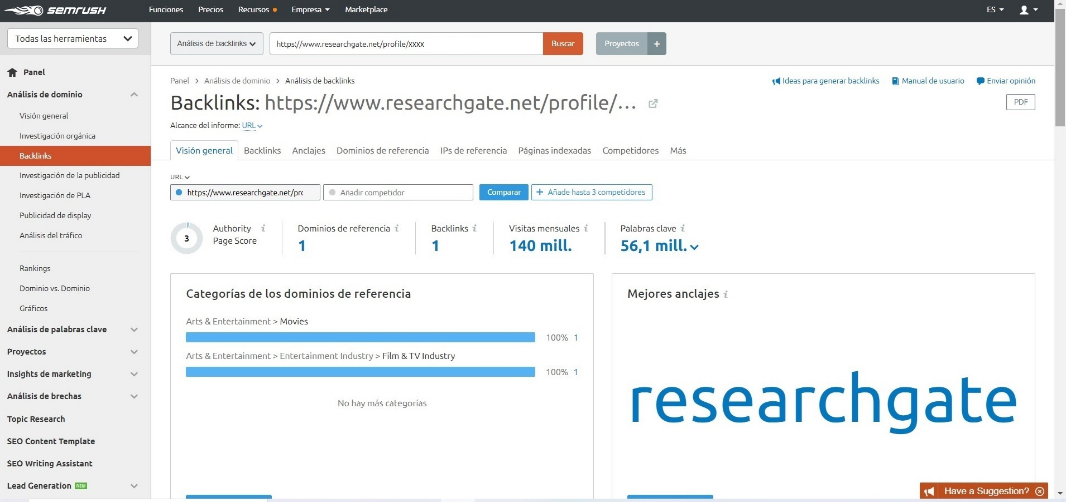
\includegraphics[width=0.95\textwidth]{Fig01.png}
 \caption{Datos de tráfico del perfil analizado en ResearchGate.}
 \label{Fig01}
 \source{propia (segundo trimestre de 2020).}
\end{figure}

\begin{figure}[htbp]
 \centering
 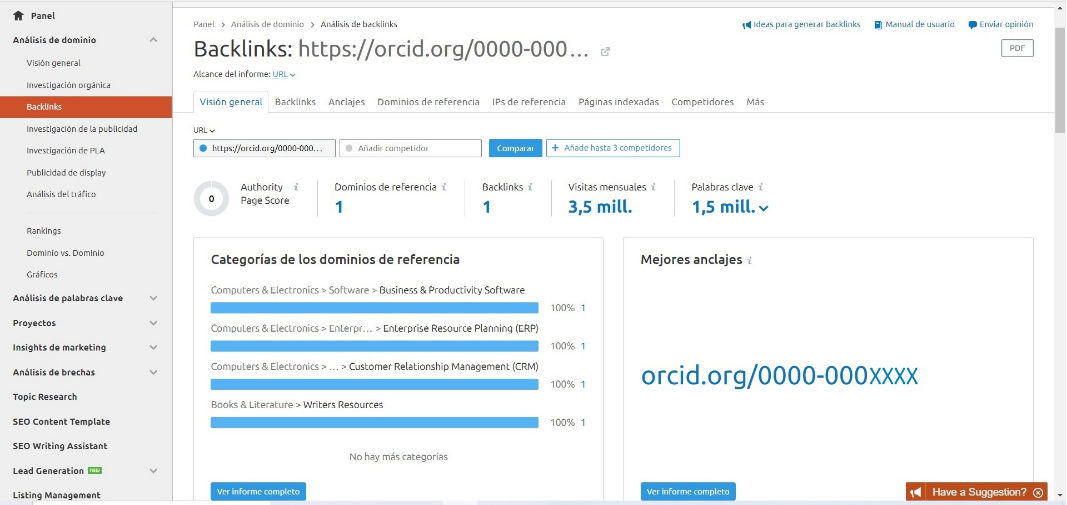
\includegraphics[width=0.95\textwidth]{Fig02.png}
 \caption{Datos de tráfico del perfil analizado en ORCID.}
 \label{Fig02}
 \source{propia (segundo trimestre de 2020).}
\end{figure}

\begin{figure}[htbp]
 \centering
 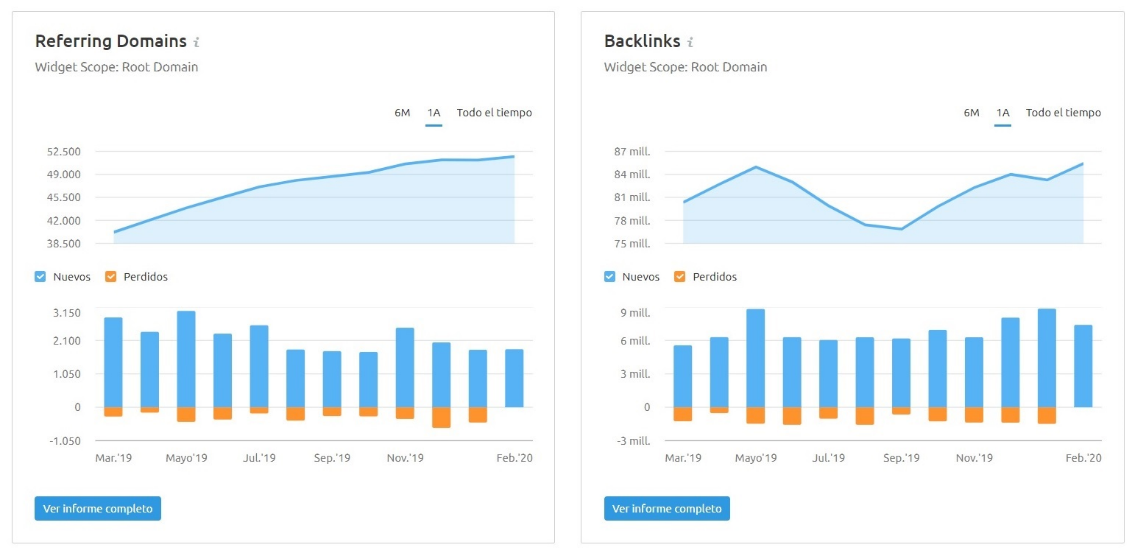
\includegraphics[width=0.95\textwidth]{Fig03.png}
 \caption{Porcentajes de pérdida (naranja) y nuevos usuarios (azul) en Directorio EXIT.}
 \label{Fig03}
 \source{propia (segundo trimestre de 2020).}
\end{figure}

\begin{figure}[htbp]
 \centering
 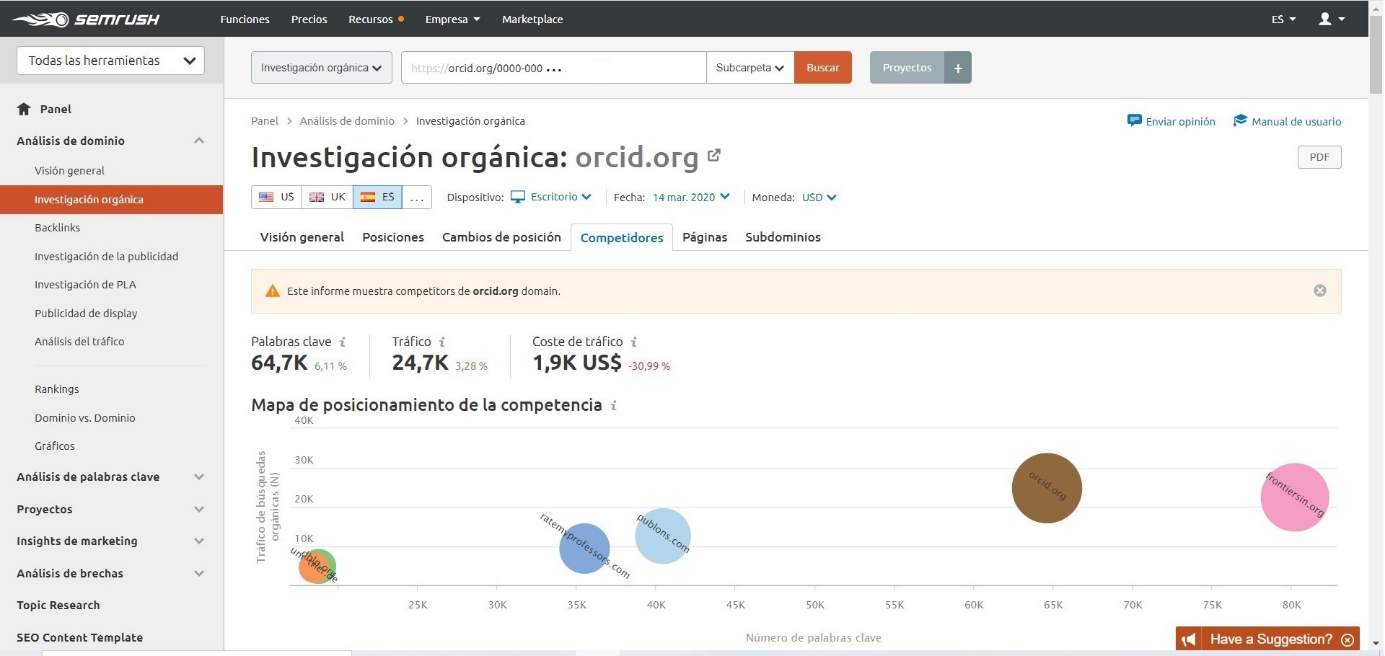
\includegraphics[width=0.95\textwidth]{Fig04.png}
 \caption{Principales competidores de ORCID en dato SemRush.}
 \label{Fig04}
 \source{propia (segundo trimestre de 2020).}
\end{figure}

Efectivamente se constata la afirmación de \textcite{sule_alonso_mk-2.0:_2010} % Sulé y Prieto (2010) 
cuando señalan que las posibilidades de encontrar a un usuario tipo en la Red ―en este caso a usuarios interesados en las temáticas abordadas por nuestro sujeto de estudio para incrementar el volumen de citas recibidas a sus trabajos de investigación― son significativas. El volumen de visitas a los perfiles abiertos, es impensable en el mundo analógico.

La herramienta más representativa de la Web 2.0 son las redes sociales \cite[p. 123]{arroyo-almaraz_community_2018} y las científicas no son una estepción.

Además, del análisis cuantitativo se extrae que la tendencia es al alza en toda la secuencia temporal analizada. En todos los perfiles abiertos el tráfico se incrementa de modo progresivo desde enero de 2019 al mes de marzo de 2020, con cifras totales muy importantes ―ver \Cref{Fig01,Fig02}―.

Se observan picos de interés que coinciden con la actividad generada en dichas plataformas y/o con algunas de las acciones colaterales diseñadas ―esto es, presencia en congresos, participación activa en listas de distribución, formación, establecimiento de nuevas alianzas, envíos de email, etcétera―, por lo que las actividades diseñadas sí parecen fructuosas.

En ORCID, Google Scholar y ResearchGate el tráfico en Estados Unidos es superior al tráfico España, aun cuando el sujeto del muestreo es de esta segunda nacionalidad, pudiendo parecer que es más habitual el acceso a estas herramientas en el primer país frente al segundo.
El porcentaje de pérdida es pequeño (\Cref{Fig03}) con lo que parece que la normalización de la firma, desde el inicio de la carrera pública del investigador, si arroja resultados positivos.

Para sorpresa del investigado, su segundo apellido es más importante como puerta de entrada que el primero, cuestión a tener en cuenta de cara a una posible normalización de la firma en entornos anglosajones ―en el ámbito hispánico la identidad formal de una personal se conforma a partir de su nombre de pila y sus apellidos, primero y principal el paterno, segundo y a continuación el materno―.

SemRush también proporciona los nombres de los principales competidores de cada dominio (\Cref{Fig04}), un elemento a monitorear para adquirir presencia en nuevos entornos que cobran actualidad y relevancia.

En la entrevista personal ―análisis cualitativo, posterior al 1 de marzo de 2020― el sujeto objeto del estudio manifiesta inexperiencia y falta de tiempo como principales dificultades en el desarrollo efectivo de la estrategia planificada. Dos cuestiones importantes que podrían explicar los picos en la atención. 

Así mismo, anota como cuestiones pendientes: la presentación a reconocimientos, que efectivamente incrementarían la visibilidad y prestigio de su perfil entre la comunidad científica; la creación de eventos propios y/o la colaboración activa en la realización de otros; acción que se asocia directamente a la mejora de sus capacidades sociales, actualmente limitadas por su timidez; seguir publicando y hacerlo con calidad en temas que interesen, con lo que podría también realizar pequeñas notas de prensa sobre los resultados de investigación ―frecuente ya en ámbitos como el sanitario y tecnológico―; ser ágil en el manejo de las redes sociales que se han abierto y no perder el interés por su actualización permanente; mejorar la formación en idiomas para abarcar más redes de confianza entre colegas que estén interesados en sus mismas líneas de investigación; entre otras.

\begin{quote}
    [E]n este nuevo contexto, la fase de difusión se caracteriza por el uso del entorno digital para visibilizar y promocionar la actividad profesional (experiencia, proyectos, etc.), la producción científica y, en general, los logros académicos. \cite[p. 70]{siso_calvo_plataformas_2020}.
\end{quote}

En términos generales se cumplen los objetivos señalados al inicio de la investigación. El sujeto tiene presencia, como mínimo, en ORCID, Google Scholar, Publons, ReaserchGate, Academia.edu y Mendeley. Tras el testeo con SemRush, se verifica un incremento en el número de visitas a los perfiles abiertos. Se observa, en toda la secuencia temporal, una tendencia al alza en el flujo de visitas a las plataformas de identificación de perfiles de investigador señaladas. Finalmente, las acciones ejecutadas tienen su reflejo en picos de atención.

Como contrapartida, el Índice H del investigador es todavía pequeño y la interacción en la Red por parte de terceros, muy limitada.

Parece que las plataformas elegidas para la apertura y presencia del investigador en la Red están aún de plena vigencia, destacando ReaserchGate, ORCID y Google Scholar por tráfico web, y en esa línea se le emplaza al sujeto a seguir trabajando.

\section{Discusión y conclusiones}\label{sec-discussao}
El nuevo modo de hacer marketing, junto a los nuevos hábitos de consumo de medios, “[c]onllevan inseparablemente una nueva forma de comunicarse con el consumidor” \cite[p. 14]{banos_gonzalez_comunicaciones_2017}. 

La hipótesis de investigación ‘una presencia activa y bien planificada en Internet mejora la visibilidad del investigador, también en el mundo analógico’ se constata matemáticamente veraz; y se ratifica con la entrevista personal y el análisis cualitativo de lo expresado por el sujeto de estudio. Además de la relevancia que ha cobrado a lo largo de todo este año el entorno de trabajo digital y la comunicación en red a causa del nuevo coronavirus, el SARS-CoV-2. 

\textcite[p. 71]{zelada_covid-19_2021}, consultora de Deloitte ―una de las llamadas Big Four (``Cuatro Grandes Auditoras'') junto a PricewaterhouseCoopers, Ernst \& Young y KPMG― señala a la COVID-19 como un acelerador de la transformación digital y añade, "[l]os desafíos que está presentando esta crisis brinda una oportunidad para que las organizaciones evolucionen a una nueva realidad donde predomina lo digital". Esto, que ella señala en el plano económico, es perfectamente extensible al personal. 
\textcite{siso_calvo_plataformas_2020} advierten que ``[l]as plataformas digitales ofrecen a los académicos la oportunidad de personal branding, teniendo en cuenta que la comunicación académica y la difusión consiste también en hacerse visible a uno mismo como investigador y no solo la producción científica''. 

El artículo aborda un tema de especial relevancia. La necesidad del investigador de hacerse visible aprovechando las ventajas de Internet, y haciendo un buen uso de las herramientas y plataformas digitales actualmente disponibles ―y en aumento― para divulgar el conocimiento producido. 

Esta es una de las vertientes inherentes a la propia “dictadura” de las métricas de evaluación, que acompañan al archi-discutido Factor de Impacto, y su legitimación para ser reflejo de la calidad de lo conocido e investigado.
También en la Ciencia, como en la Academia, pasa a ser crucial estar vivo, hacerse ver; y desde luego porque a mayor difusión del conocimiento producido, mayor visibilidad y potencialidad de citación, que a su vez sirve para legitimar la posición de los investigadores en un mundo científico cada vez más saturado de sobreproducción científica y de frustración. Por no hablar de la financiación de nuevos proyectos, sexenios, etcétera, dónde una vez más el reconocimiento en forma de cita bibliográfica, es base de ponderación.

En este contexto, se valora el papel del acceso abierto en la democratización del conocimiento, y lo que la propia democratización y apertura acarrea de nuevo para los investigadores, que deben subirse a esa rueda como a la de un hámster situada permanentemente en paralelo a la vida cotidiana y a los quehaceres ordinarios.

Bien es verdad, que “[a]medida que aumenta el acceso a nuestros datos digitales, también lo hacen las preocupaciones culturales, las ansiedades y los movimientos proteccionistas relacionados en torno a la privacidad digital” \cite[p. 155]{holt_privacy_2015}. Como recogen los autores \cite{holt_privacy_2015}, los reguladores enfrentan una serie de retos que a menudo desafían las resoluciones legales, ya que la infraestructura de Internet se extiende más allá de las fronteras nacionales. En consecuencia, no existe un régimen unificado en el que se proteja la privacidad, sino más bien una serie de enfoques nacionales por los que deben navegar todos los usuarios y proveedores de contenido de Internet; y ello, efectivamente, puede ralentizar o repeler la entrada de nuevos actores a la difusión web de contenidos de investigación, más partidarios de dejar en manos de terceros ―la comunicación tradicional y al editor― el prestigio de su nombre. Sin embargo, lo que no se había recorrido hasta ahora, es camino andado con la pandemia.

En esta segunda investigación, que arranca como consecuencia de una primera en la que se analizaron los perfiles de 2257 investigadores del área de Comunicación y su comportamiento en la Red \cite{mandia-rubal_implantacion_2019}; se pretendía profundizar en el estudio de un caso particular, monitorizando el volumen de visitas a los perfiles web abiertos después de poner en práctica estrategias propias del marketing digital y el posicionamiento web, o SEO.

En 2019 un grupo de científicos publicaba los resultados de un experimento cercano a la física cuántica que probaba que la realidad no existe hasta que es medida, al menos no la realidad en una escala cuántica \cite{proietti_experimental_2019}. Si esto es así, el hecho de haber publicado ―de existir esa información en algún lugar― no garantiza su existencia para todo el resto del mundo.

No es sólo que el trabajo que se realice tenga calidad y publicarlo, por supuesto ambos elementos indispensables en la comunicación de la ciencia ―como también lo son en el marketing―; tanto como saber atraer la atención hacia su contenido. De eso trata este artículo, y también de las herramientas utilizadas y los resultados obtenidos.
Como recordaba Castells, ya en 2011, el liderazgo existe. Está en la Red.

La Red es, por el momento, la única alternativa a la presencialidad, y al igual que no se descuidaba la presencia física en los eventos analógicos, no debe el investigador de hoy descuidar su identidad digital, única puerta de entrada en muchos casos a su perfil como profesional.

\printbibliography\label{sec-bib}

\end{document}
